\documentclass[12pt]{article}

\usepackage[margin=1in]{geometry}
\usepackage{amsmath,amsthm,amssymb}

\newcommand{\N}{\mathbb{N}}
\newcommand{\Z}{\mathbb{Z}}
\newcommand{\homeworkheader}[2]{
  \title{Homework #1}
  \author{Erich Menge (X.500: menge053, Student ID: 4624713) \\
  #2}
  \maketitle
}

\newenvironment{problem}[1]{
  \ignorespaces
  \section*{Problem #1}
}{
  \ignorespacesafterend
}

\newcommand{\classnameandsection}{CSCI 4707 Practice of Database Systems}

\usepackage{pgf}
\usepackage{tikz}
\usetikzlibrary{arrows,automata}

\sethomeworknumber{2}

\begin{document}
\homeworkheader{\classnameandsection}

\begin{problem}{1}
  Do Exercise 1.28 parts c from the book.
  \begin{solution}
    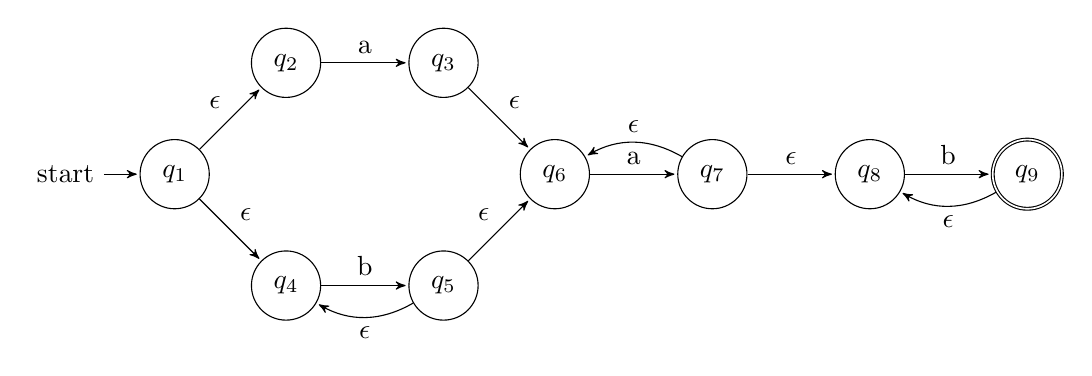
\begin{tikzpicture}[>=stealth',shorten >=1pt,auto,node distance=2cm]
      \node[initial, state] (q1){$q_1$};
      \node[state] [above right of=q1] (q2){$q_2$};
      \node[state] [below right of=q1] (q4){$q_4$};
      \node[state] [right of=q2] (q3){$q_3$};
      \node[state] [right of=q4] (q5){$q_5$};
      \node[state] [below right of=q3] (q6){$q_6$};
      \node[state] [right of=q6] (q7){$q_7$};
      \node[state] [right of=q7] (q8){$q_8$};
      \node[state, accepting] [right of=q8] (q9){$q_9$};

      \path[->]
        (q1)
          edge node{$\epsilon$}(q2)
          edge node{$\epsilon$}(q4)
        (q2)
          edge node{a}(q3)
        (q3)
          edge node{$\epsilon$}(q6)
        (q4)
          edge node{b}(q5)
        (q5)
          edge[bend left] node{$\epsilon$}(q4)
          edge node{$\epsilon$}(q6)
        (q6)
          edge node{a}(q7)
        (q7)
          edge node{$\epsilon$}(q8)
          edge [bend right] node[swap]{$\epsilon$}(q6)
        (q8)
          edge node{b}(q9)
        (q9)
          edge[bend left] node{$\epsilon$}(q8)
      ;

    \end{tikzpicture}

  \end{solution}
\end{problem}

\begin{problem}{2}
  Do Exercise 1.21 part b from the book.
\end{problem}

\begin{problem}{3}
  Do Problem 1.41 from the book. The most obvious way to solve this problem is by is by showing how to construct a finite automaton accepting the perfect shuffle of A and B from dfas accepting A and B.
\end{problem}

\begin{problem}{4}
  Do Problem 1.46 parts c from the book.
\end{problem}

\begin{problem}{5}
  Do Problem 1.47 from the book. You may find it useful to use the fact that regular languages are closed under complementation.
\end{problem}

\begin{problem}{6}
  Let $\Sigma$ = \{0,1\}
  \begin{enumerate}
    \item Let A = $\{ 0^ku0^k | k \ge 1$ and $u \in \Sigma^* \}$ Show that A is regular \\
    \item Let B = $\{ 0^k1u0^k | k \ge 1$ and $u \in \Sigma^* \}$. Show that B is not regular.
  \end{enumerate}
\end{problem}

\begin{problem}{7}
  Define the avoids operation on languages A and B to be \\
  \newline\indent avoids(A,B) = $\{ w | w \in$ A and $w$ does not contain any string in B as a substring $\}$ \\
  \newline Prove that the class of regular languages is closed under the avoids operation.
\end{problem}


\end{document}
